% Seminar thesis template (LaTeX) -- Statistics Seminar, KU Eichstaett-Ingolstadt
% Works on Overleaf (compiler: pdfLaTeX) and with a local LaTeX installation.

\documentclass[12pt, a4paper]{scrartcl}

% ---- Formal requirements: 12 pt, 1.5 line spacing, 2.5 cm margins ----------
\usepackage[margin=2.5cm]{geometry}
\usepackage[onehalfspacing]{setspace}

% ---- Fonts and language --------------------------------------------------------
\usepackage[T1]{fontenc}
\usepackage[utf8]{inputenc}
\usepackage{lmodern}
\usepackage[english]{babel}
\usepackage{csquotes}

% ---- Mathematics, tables, figures -----------------------------------------
\usepackage{amsmath, amssymb, amsthm}
\usepackage{booktabs}
\usepackage{graphicx}

% ---- Code snippets: single-spaced, small font --------------------------------
\usepackage{listings}
\lstset{
  language     = R,          % change to Python if you use Python
  basicstyle   = \small\ttfamily\linespread{1}\selectfont,
  frame        = single,
  columns      = fullflexible,
  keepspaces   = true,
  showstringspaces = false
}

% ---- Literature (author-year citations) --------------------------------------
\usepackage[style=authoryear, backend=biber]{biblatex}
\addbibresource{references.bib}

\usepackage[colorlinks=true, linkcolor=blue, citecolor=blue, urlcolor=blue]{hyperref}

% ---- Results produced by R/simulation.R ---------------------------------------
\newcommand{\nreps}{5000}


% ---- Title page ---------------------------------------------------------------
\title{Title of Your Seminar Thesis}
\subtitle{Seminar Thesis $\cdot$ Statistics Seminar $\cdot$ KU Eichstätt-Ingolstadt}
\author{Name One (Matriculation No.) \and
        Name Two (Matriculation No.) \and
        Name Three (Matriculation No.)}
\date{\today}

\begin{document}

\maketitle

\begin{abstract}
  Summarize your thesis in a few sentences: Which method do you study,
  what are its key assumptions, and what did your simulation study reveal
  about when the method works and when it fails?
\end{abstract}

\tableofcontents
\newpage

% Page limit: 8--12 pages for the main text (Sections 1 to 5), including
% figures and tables. Title page, table of contents, references, and
% appendix do not count.

\section{Introduction}

\emph{Write this part at the end.} What problem does the method solve, and
where is it used? What is the goal of your thesis, and how is it structured?

\section{Main Part 1: The Model and the Method}

Describe the data and the statistical model, and list all assumptions of the
method. Explain each assumption in words.

Define the method with formulas, explain the idea behind it, and state its most
important theoretical properties. Explain which assumptions are needed for
them. Cite your sources, e.g., \textcite{Silverman1986} or
\parencite{Silverman1986}.

Show code only when it helps the reader to understand the method, and keep such
snippets short:

\begin{lstlisting}
ci_mean <- function(x, level = 0.95) {
  q <- qt(1 - (1 - level) / 2, df = length(x) - 1)
  mean(x) + c(-1, 1) * q * sd(x) / sqrt(length(x))
}
\end{lstlisting}

\section{Main Part 2: Applying the Method to Artificial Data}

Describe the design of your simulation study: the data generating processes,
which assumption each of them violates, the sample sizes, the number of
replications, and the performance measures.

The following example studies the coverage probability of the classical 95\%
confidence interval for the mean, which assumes normally distributed data.
Table~\ref{tab:coverage} and Figure~\ref{fig:coverage} show the results based
on \nreps{} Monte Carlo replications.

\begin{table}[htbp]
  \centering
  \caption{Empirical coverage probabilities of the 95\% confidence interval for the mean.}
  \label{tab:coverage}
  \begin{tabular}{lrrrrr}
\toprule
Distribution & $n = 10$ & $n = 25$ & $n = 50$ & $n = 100$ & $n = 250$ \\
\midrule
Normal (baseline) & 0.954 & 0.956 & 0.955 & 0.946 & 0.947 \\
Exponential (skewed) & 0.900 & 0.924 & 0.937 & 0.939 & 0.946 \\
Log-normal (very skewed) & 0.707 & 0.769 & 0.829 & 0.845 & 0.884 \\
\bottomrule
\end{tabular}

\end{table}

\begin{figure}[htbp]
  \centering
  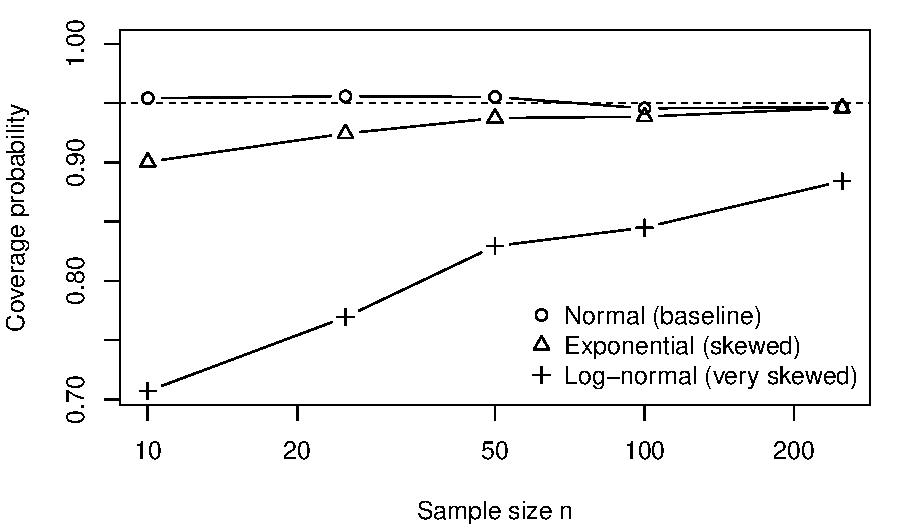
\includegraphics[width=\textwidth]{results/coverage.pdf}
  \caption{Empirical coverage probabilities. The dashed line marks the nominal
  level of 95\%.}
  \label{fig:coverage}
\end{figure}

Interpret the results: When can a user rely on the method? What should a user
watch out for in practice?

\section{Main Part 3: Applying the Method to Real Data}

Describe the data set, apply the method, and interpret the results. Are the
assumptions plausible for these data? What does your simulation study tell you
about how much you can trust the results?

\section{Conclusion}

\emph{Write this part at the end.} Summarize your main findings and give
practical advice: When should a user apply the method, and what should a user
be careful about?

\printbibliography[heading=bibintoc, title=References]

\appendix

\section{Appendix}

Additional figures, tables, or proofs can go here. The full code is not printed
here, but submitted as separate files (see the README).

\end{document}
